\documentclass[aspectratio=169,11pt]{beamer}
\usepackage[T1]{fontenc}
\usepackage{lmodern,amsmath,amssymb,mathtools,bm,booktabs,array,graphicx,tikz}
\usetikzlibrary{arrows.meta,positioning,calc,decorations.pathreplacing,patterns}
\definecolor{ink}{HTML}{17344D}\definecolor{accent}{HTML}{087E8B}\definecolor{pale}{HTML}{EDF5F5}\definecolor{gold}{HTML}{AD6B19}
\providecommand{\dd}{\,\mathrm{d}}\providecommand{\R}{\mathbb{R}}
\providecommand{\E}{\mathbb{E}}\providecommand{\Var}{\operatorname{Var}}
\providecommand{\Cov}{\operatorname{Cov}}\providecommand{\diag}{\operatorname{diag}}
\providecommand{\norm}[1]{\left\lVert#1\right\rVert}
\providecommand{\abs}[1]{\left|#1\right|}
\usefonttheme{professionalfonts}
\setbeamercolor{normal text}{fg=black,bg=white}
\setbeamercolor{frametitle}{fg=ink,bg=white}
\setbeamercolor{title}{fg=ink}\setbeamercolor{structure}{fg=accent}
\setbeamercolor{block title}{fg=ink,bg=pale}\setbeamercolor{block body}{fg=black,bg=pale!40}
\setbeamercolor{alerted text}{fg=accent}
\setbeamerfont{frametitle}{size=\Large,series=\bfseries}
\setbeamerfont{title}{size=\LARGE,series=\bfseries}
\setbeamertemplate{navigation symbols}{}
\setbeamersize{text margin left=.7cm,text margin right=.7cm}
\setbeamertemplate{frametitle}{\vspace{.18cm}\insertframetitle\par\vspace{.1cm}{\color{accent}\hrule height .6pt}\vspace{.12cm}}
\newcommand{\notestarget}{notes.pdf}\newcommand{\noteslabel}{Notes}
\setbeamertemplate{footline}{\hspace{.7cm}\color{ink}\scriptsize Mathematical Modeling\quad\href{\notestarget}{\noteslabel}\hfill\insertframenumber\,/\,\inserttotalframenumber\hspace{.7cm}\vspace{.18cm}}
\setbeamercovered{invisible}
\hypersetup{pdfauthor={Zan Ahmad},pdftitle={Cable equations and propagation through a branch},pdfpagemode=UseNone}
\begin{document}
\begin{frame}[plain]\vfill
{\small\color{accent} Mathematical Modeling \quad Lecture 10}\par\medskip
{\raggedright\hyphenpenalty=10000\exhyphenpenalty=10000\LARGE\bfseries\color{ink} Cable equations and propagation through a branch}\par\bigskip
Zan Ahmad\par\smallskip
{\small Fall 2024}\par\vfill\end{frame}
\renewcommand{\notestarget}{notes.pdf\#note-axial-conduction-and-local-charge-conservation}
\begin{frame}[t,fragile,label=slide-axial-ohm-law]{Axial Ohm law}
\[I_a=-\frac{\pi a^2}{\rho}\partial_xV.\]\pause{} Cross-sectional area determines axial conduction; membrane area determines capacitive and ionic currents.
\end{frame}
\renewcommand{\notestarget}{notes.pdf\#note-axial-conduction-and-local-charge-conservation}
\begin{frame}[t,fragile,label=slide-charge-conservation-on-a-short-segment]{Charge conservation on a short segment}
\[-\partial_xI_a=2\pi a(C\partial_tV+I_{\mathrm{ion}}-I_{\mathrm{app}}).\]\pause{} Axial current lost along the segment must cross or charge its membrane.
\end{frame}
\renewcommand{\notestarget}{notes.pdf\#note-axial-conduction-and-local-charge-conservation}
\begin{frame}[t,fragile,label=slide-the-active-cable-equation]{The active cable equation}
\[C\partial_tV=\frac a{2\rho}\partial_{xx}V-I_{\mathrm{ion}}+I_{\mathrm{app}}.\]\pause{} Local gate equations accompany every spatial point.\par\medskip This is a reaction--diffusion system, not the classical wave equation.
\end{frame}
\renewcommand{\notestarget}{notes.pdf\#note-passive-length-and-time-scales}
\begin{frame}[t,fragile,label=slide-passive-membrane-scales]{Passive membrane scales}
For $u=V-E_L$:\[\tau_m u_t=\lambda^2u_{xx}-u,\quad\tau_m=C/g_L,\quad\lambda^2=a/(2\rho g_L).\]\pause{} Time relaxation and steady spatial attenuation are different observables.
\end{frame}
\renewcommand{\notestarget}{notes.pdf\#note-passive-length-and-time-scales}
\begin{frame}[t,fragile,label=slide-a-sealed-cable-exact-benchmark]{A sealed-cable exact benchmark}
\[u(x,t)=B\cos(kx)e^{-(Dk^2+g_L/C)t},\quad k=j\pi/\ell.\]\pause{}\[D=a/(2\rho C),\qquad u_x(0,t)=u_x(\ell,t)=0.\]
\end{frame}
\renewcommand{\notestarget}{notes.pdf\#note-a-conservative-network-discretization}
\begin{frame}[t,fragile,label=slide-shared-edge-currents]{Shared edge currents}
\[K_{ij}=\frac{\pi r_{ij}^2}{\rho\Delta x_{ij}},\qquad I_{i\to j}=K_{ij}(V_i-V_j).\]\pause{} $K$ is in mS, $V$ in mV, and total edge current in $\mu\mathrm A$.
\end{frame}
\renewcommand{\notestarget}{notes.pdf\#note-a-conservative-network-discretization}
\begin{frame}[t,fragile,label=slide-membrane-area-assigned-to-nodes]{Membrane area assigned to nodes}
\[A_i=\sum_{j\sim i}\pi r_{ij}\Delta x_{ij},\qquad M_i=CA_i.\]\pause{} Each endpoint receives half an edge lateral area.\par\medskip A junction receives contributions from every incident edge.
\end{frame}
\renewcommand{\notestarget}{notes.pdf\#note-a-conservative-network-discretization}
\begin{frame}[t,fragile,label=slide-the-finite-volume-voltage-balance]{The finite-volume voltage balance}
\[M_i\dot V_i+A_iI_{\mathrm{ion},i}+\sum_jK_{ij}(V_i-V_j)=I_{\mathrm{app},i}.\]\pause{} Every term is a total current; membrane densities must be multiplied by area.
\end{frame}
\renewcommand{\notestarget}{notes.pdf\#note-junction-storage-and-the-summed-current-budget}
\begin{frame}[t,fragile,label=slide-a-charging-branch-junction]{A charging branch junction}
\[I_C=0.006-0.002-0.001-0.001=0.002\,\mu\mathrm A.\]\pause{}\[\dot V=0.002/0.0002=10\,\mathrm{mV/ms}.\] Over $0.01\,\mathrm{ms}$, the initial-rate estimate is $0.1\,\mathrm{mV}$.
\end{frame}
\renewcommand{\notestarget}{notes.pdf\#note-junction-storage-and-the-summed-current-budget}
\begin{frame}[t,fragile,label=slide-cancellation-in-the-global-current-budget]{Cancellation in the global current budget}
\[\frac{\dd}{\dd t}\sum_iM_iV_i+\sum_iA_iI_{\mathrm{ion},i}=\sum_iI_{\mathrm{app},i}.\]\pause{} Internal axial currents cancel pairwise.\par\medskip Weighted charge, not unweighted voltage sum, enters the balance.
\end{frame}
\renewcommand{\notestarget}{notes.pdf\#note-the-coupled-implicit-voltage-solve}
\begin{frame}[t,fragile,label=slide-the-graph-laplacian]{The graph Laplacian}
\[(LV)_i=\sum_jK_{ij}(V_i-V_j),\qquad L\mathbf1=0.\]\pause{}\[z^TLz=\sum_{\{i,j\}}K_{ij}(z_i-z_j)^2\geq0.\]
\end{frame}
\renewcommand{\notestarget}{notes.pdf\#note-the-coupled-implicit-voltage-solve}
\begin{frame}[t,fragile,label=slide-an-implicit-coupled-voltage-step]{An implicit coupled voltage step}
After the exact frozen-voltage gate update, set $G_i=\sum_jg_{ij}$ and $b_i=\sum_jg_{ij}E_j$.\pause{}\[\left(M/\Delta t+L+D_A\operatorname{diag}(G)\right)V^{k+1}=MV^k/\Delta t+D_Ab+I_{\mathrm{app}}.\]
\end{frame}
\renewcommand{\notestarget}{notes.pdf\#note-the-coupled-implicit-voltage-solve}
\begin{frame}[t,fragile,label=slide-positive-definiteness-and-a-unique-solve]{Positive definiteness and a unique solve}
$M_i>0$, $\Delta t>0$, and $G_i\geq0$ give\[z^T(M/\Delta t+L+D_A\operatorname{diag}(G))z>0\quad(z\ne0).\]\pause{} The matrix solve is uniquely defined; stability does not remove time-discretization error.
\end{frame}
\renewcommand{\notestarget}{notes.pdf\#note-the-coupled-implicit-voltage-solve}
\begin{frame}[t,fragile,label=slide-elimination-along-a-tree]{Elimination along a tree}
Eliminate a leaf $i$ attached to parent $p$:\[d_p\leftarrow d_p-K_{ip}^2/d_i,\qquad r_p\leftarrow r_p+K_{ip}r_i/d_i.\]\pause{} Solve the root, then recover child voltages in reverse order.
\end{frame}
\renewcommand{\notestarget}{notes.pdf\#note-a-branched-neuronal-experiment}
\begin{frame}[label=slide-the-synthetic-branched-experiment-figure]{The synthetic branched experiment}
\centering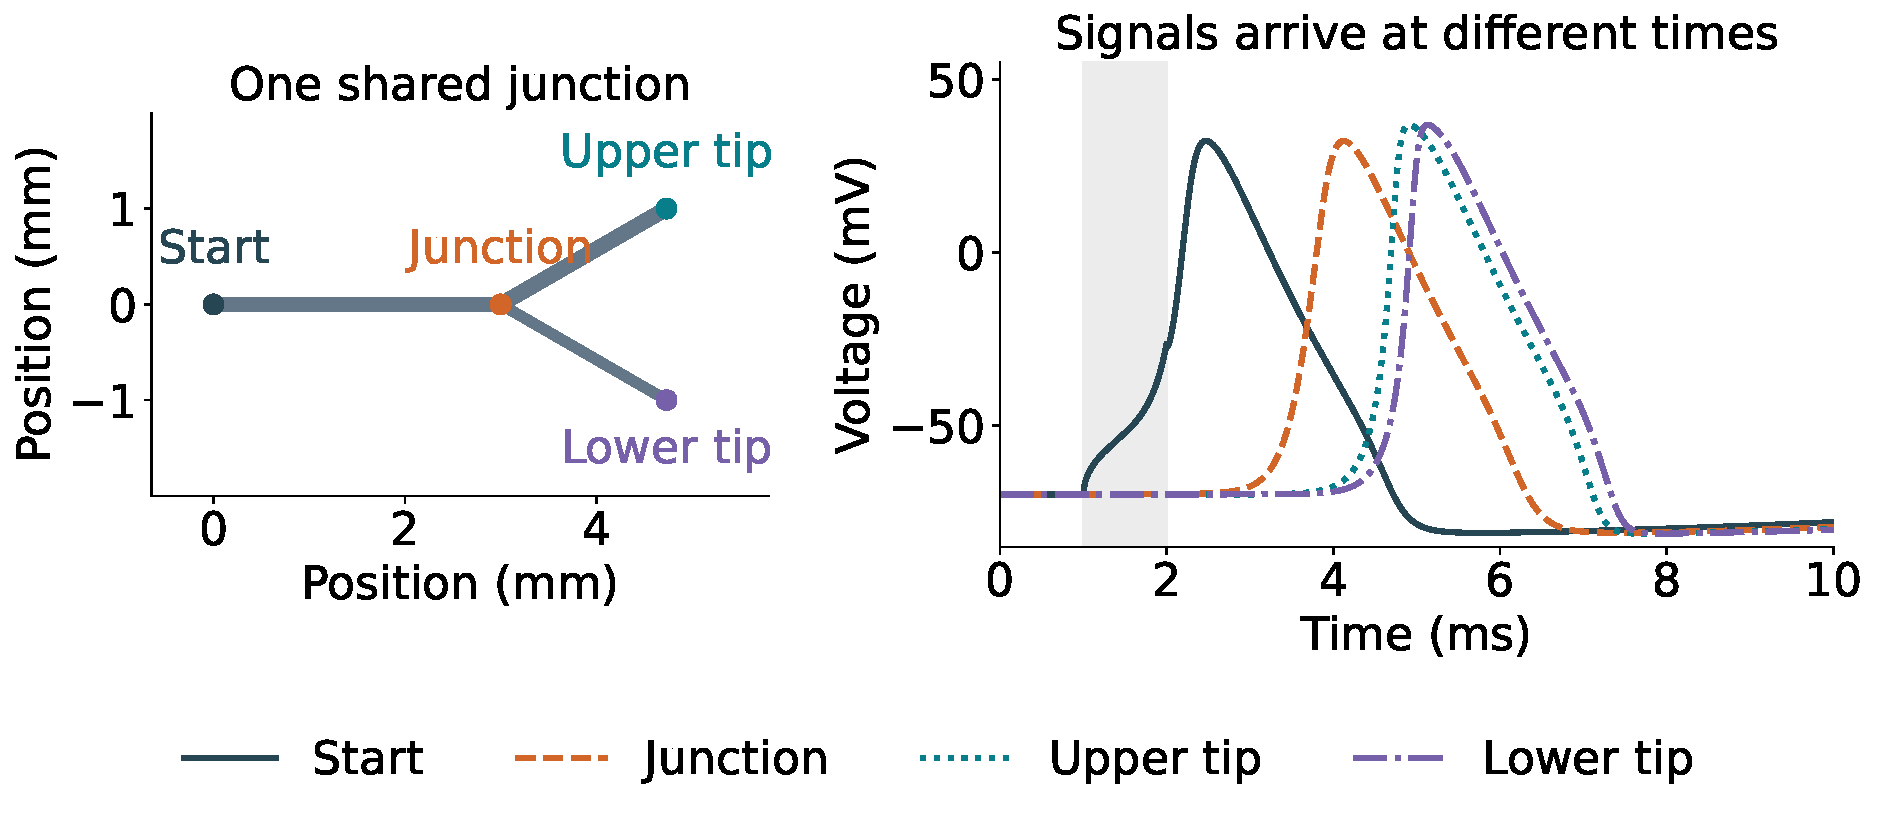
\includegraphics[width=.98\linewidth,height=.69\textheight,keepaspectratio]{branched-probes.pdf}\end{frame}
\renewcommand{\notestarget}{notes.pdf\#note-a-branched-neuronal-experiment}
\begin{frame}[t,fragile,label=slide-the-synthetic-branched-experiment]{The synthetic branched experiment}
Trunk $3\,\mathrm{mm}$; daughters $2\,\mathrm{mm}$ each.\par Radii: $5,5,3.5\,\mu\mathrm m$.\pause{}\par\medskip One shared junction, $71$ nodes, input $0.006\,\mu\mathrm A$ on $[1,2)\,\mathrm{ms}$.
\end{frame}
\renewcommand{\notestarget}{notes.pdf\#note-a-branched-neuronal-experiment}
\begin{frame}[label=slide-time-traces-and-spatial-snapshots-figure]{Time traces and spatial snapshots}
\centering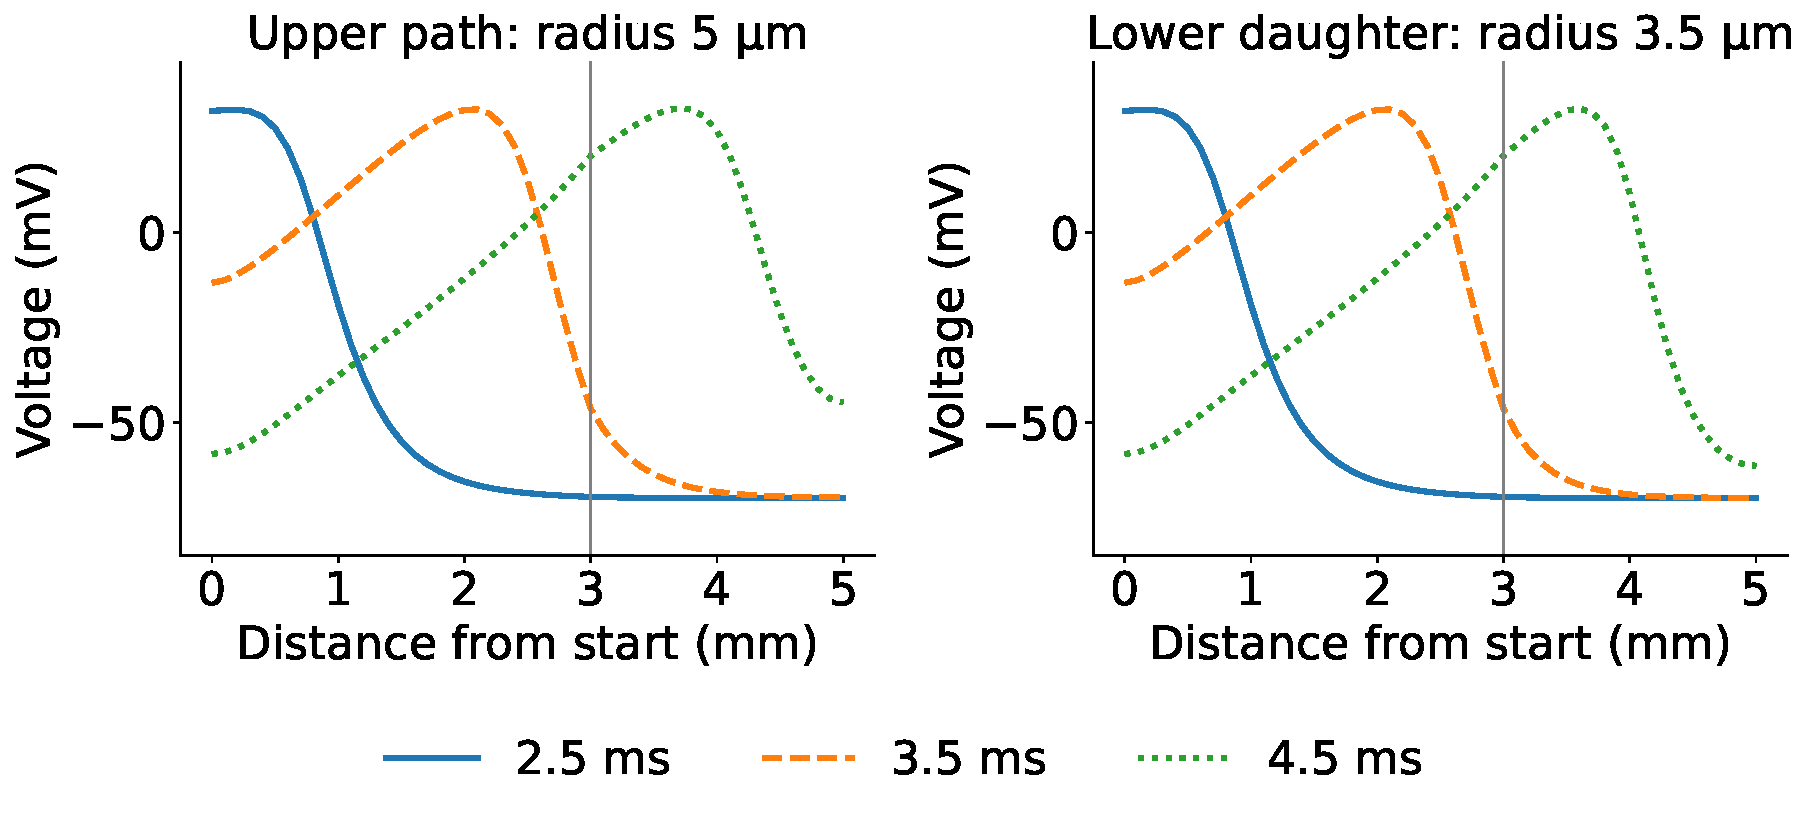
\includegraphics[width=.98\linewidth,height=.69\textheight,keepaspectratio]{traveling-profiles.pdf}\end{frame}
\renewcommand{\notestarget}{notes.pdf\#note-a-branched-neuronal-experiment}
\begin{frame}[t,fragile,label=slide-time-traces-and-spatial-snapshots]{Time traces and spatial snapshots}
A trace fixes position; a snapshot fixes time.\pause{}\par\medskip Both path panels share the same trunk.\par Snapshots: $2.5$, $3.5$, $4.5\,\mathrm{ms}$.\par\medskip Local ionic feedback regenerates the signal as axial current spreads.
\end{frame}
\renewcommand{\notestarget}{notes.pdf\#note-arrival-measurements-and-independent-numerical-checks}
\begin{frame}[t,fragile,label=slide-threshold-based-arrival-and-speed]{Threshold-based arrival and speed}
Use the first upward $0\,\mathrm{mV}$ crossing at both probes.\pause{}\[v_{\mathrm{avg}}=\frac{2\,\mathrm{mm}}{4.692-3.799\,\mathrm{ms}}\simeq2.24\,\mathrm{m/s}.\] Arrival from stimulus onset includes initiation delay.
\end{frame}
\renewcommand{\notestarget}{notes.pdf\#note-arrival-measurements-and-independent-numerical-checks}
\begin{frame}[t,fragile,label=slide-a-discrete-current-budget-residual]{A discrete current-budget residual}
\[\sum_iM_i\Delta V_i+\Delta t\sum_iA_i(G_iV_i^{k+1}-b_i)-\Delta t\sum_iI_{\mathrm{app},i}=0.\]\pause{} Use the conductances and new voltages actually used by the numerical scheme.
\end{frame}
\renewcommand{\notestarget}{notes.pdf\#note-arrival-measurements-and-independent-numerical-checks}
\begin{frame}[t,fragile,label=slide-separate-tests-of-algebra-space-and-time]{Separate tests of algebra, space, and time}
Tree solve versus dense solve: algebra.\par Passive cosine versus continuum solution: space and time.\par Exact discrete-system evolution: isolated time error.\pause{}\par\medskip Active arrival refinement at one mesh does not establish active spatial convergence.
\end{frame}
\renewcommand{\notestarget}{notes.pdf\#note-arrival-measurements-and-independent-numerical-checks}
\begin{frame}[t,fragile,label=slide-model-evidence-for-a-propagated-signal]{Model evidence for a propagated signal}
Geometry, stimulus, channel laws, and recording locations determine the experiment.\pause{}\par\medskip Measured waveforms are needed for biological validation.\par\medskip The current model omits extracellular gradients and holds reversal potentials fixed.
\end{frame}
\end{document}
